\documentclass[12pt,letterpaper]{article}
\usepackage{amsmath}
\usepackage{fancyhdr}
\usepackage{graphicx}
\usepackage{alltt}
\usepackage{color}
\usepackage{colortbl}
\usepackage{fullpage}
\usepackage{setspace}
\usepackage{pstricks}
\usepackage{verbatim}
\usepackage{comment}
\usepackage{framed}
\usepackage{listings}
\usepackage{longtable}
\usepackage{pdflscape}
\usepackage{multirow}
\usepackage[config=altsf]{subfig}
\usepackage[utf8]{inputenc}
\usepackage[francais]{babel}
\usepackage[plainpages=false,pdfpagelabels,hypertexnames=false]{hyperref}

%For pdf selection
\usepackage[T1]{fontenc}
\usepackage{lmodern}

%%%%% STYLE %%%%%%%
\topmargin	0in
\topskip	0in
\headheight	0in
\headsep	0in
\parindent	0in
\topsep		0in
\parskip	8pt
\floatsep	0in
%%%%%%%%%%%%%%%%%%%%

%%% SETUP HYPERLINK %%%%%
\hypersetup{
colorlinks 	= true,
linkcolor 	= black}
%%%%%%%%%%%%%%%%%%%%%%%%%

\begin{document}

%%%%%%% COMMANDS %%%%%%%%
\renewcommand{\labelitemi}{$\bullet$}
\newcommand{\unit}[1]{\ \mathrm{#1}}
\newcommand{\degree}{\ensuremath{^\circ}}
%%%%%%%%%%%%%%%%%%%%%%%%%

%%%%%%%%%%%%%%%%%%%%% PAGE TITRE %%%%%%%%%%%%%%%%%%%%%%%%%%%%%%%%%%%%
%%%%%%%%%%%%%%%%%%%%%%%%%%%%%%%%%%%%%%%%%%%%%%%%%%%%%%%%%%%%%%%%%%%%%
\thispagestyle{empty}
\begin{center}
	\vspace{20pt}
	\large{\textsc{
		Intelligence artificielle bio-inspirée\\
	}}
	\vspace{20pt}
	\large{\textsc{
		P02
	}}
	\vfill
	\begin{tabular}{ll}
      Simon Mathieu & 04 450 409 \\
      Steven Denis & 05 667 682 \\
      Michael Janelle-Montcalm & 04 526 123 \\
      Martin Provencher &	05 666 488 \\
	\end{tabular}
	\vfill
	Novembre 2009 \\
	\textbf{Université de Sherbrooke}
	\vspace{20pt}
\end{center}
\clearpage
%%%%%%%%%%%%%%%%%%%%% TABLE DES MATIÈRES %%%%%%%%%%%%%%%%%%%%%%%%%%%%
%%%%%%%%%%%%%%%%%%%%%%%%%%%%%%%%%%%%%%%%%%%%%%%%%%%%%%%%%%%%%%%%%%%%%
\begin{spacing}{0.1}
\tableofcontents
\end{spacing}
\clearpage

\section{Introduction}

\section{Analyse des données} % Steven
% Similitudes entre les canaux (redondance entre 1 et 6, on garde 6)
% Valeurs des maxima et minima sont plus grandes lors d'une chute que lors 
% d'une non-chute

\section{Hypothèses simplificatrices}

\subsection{Logique floue}

\subsection{Réseau de neurones} % Mike
% Utilisation seulement des max et min permet d'identifier les chutes

\section{Représentation de l'information}

\subsection{Logique floue}

\subsection{Réseau de neurones} % Steven
% Schéma-bloc du système
% Extraction des caractéristiques (max, min)
% Entrées et sorties (fichiers de données, sorties du script)

\section{Mise en oeuvre}

\subsection{Logique floue}

\subsection{Réseau de neurones} % Mike
% Données d'entraînement (sujet 5)
% Description de l'évolution du réseau (époques)
% Paramètres d'entraînement (momentum, learning rate)
% Ne converge pas toujours
% – Loi d’apprentissage, nombre d’unités cachées, nombre d’unités de sortie a expérimenter ;
% – Critères d’entraînement et d’évaluation ;
% – Création des ensembles d’entraînement et de test en lien avec l’apprentissage ;
% – Critère de classification et de reconnaissance.

\subsection{Algorithme génétique}

Originalement, nous voulions utiliser le nombre de piques dans le graphique de la dérivé pour détecter les chutes.
Si le graphique d'un capteur contenait un pique, il s'agit probablement d'une chute, si il en contient aucun, il 
ne s'agît pas d'une chute. Si il en contient plusieurs, il s'agit d'une récupération de chute. 

Les figures \ref{fig:chute} et \ref{fig:nonchute} montre la différence entre une chute et une récupération de chute.

\begin{figure}[htp]
\centering
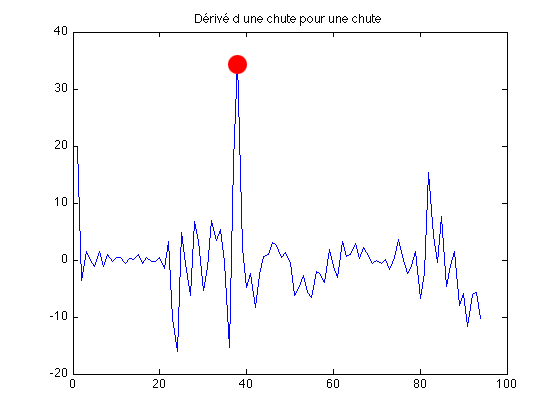
\includegraphics{image/piques_chute.png}
\label{fig:chute}
\caption{Nombre de piques pour une chute}
\end{figure}


\begin{figure}[htp]
\centering
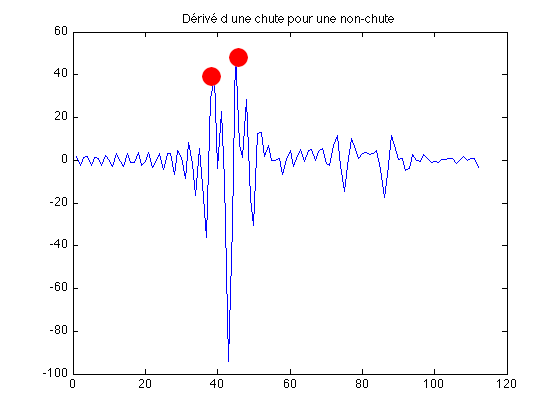
\includegraphics{image/piques_nonchute.png}
\label{fig:nonchute}
\caption{Nombre de piques pour une non-chute}
\end{figure}



Pour détecter un pique, nous utilisions une librairie matlab trouvé sur internet. La fonction de détection de pique
possède 4 paramètres permettant de contrôller quel points du graphique sont détectés comme étant des piques. 

Comme ces paramètre peuvents prendrent une très grand quantité de valeurs, il s'agissait d'un cas intéressant ou utiliser
un algorithme génétique pour trouver les valeurs optimales. 

La première étape de la mise en oueuvre fut de manuellement se créer des données d'entrainement. Nous avons donc manuellement
observé les graphiques de la dérivé de certains des capteurs et avons estimé le nombre de pique. 

Armé de ces données, nous avons ensuite définit une fonction de pertinence qui permet de calculer la distance une données est de 
la valeur réel. 

Nous avons ensuite définit une population d'individu qui se composait d'un ensemble de valeurs représentent les paramètre des la
fonction qui trouve les piques. 

La prochaine étape consiste a faire reproduire et muter les individus de notre population pour produire la prochaine génération. Après 
observation, nous avons conclus qu'il était mieux de conserver les individus d'un génération dans la prochaine. Nous gardons donc les 
cinq individus les mieux adapter. 

Le choix des individus qui se reproduisent est fait à l'aide d'une fonction aléatoire pondéré de façon a ce que les individus possèdant
des meilleurs gènes aillent une meilleur probabilité de se reproduire. 

Le speudo code de notre algorithme est:

\begin{verbatim}
pop = InitPopulation

FOR n generation
  fitenesses = CalculateFitness pop
  breeders = SelectBreeders pop
  pop = Reproduce breeders
  pop = Mutate pop

\end{verbatim}


\section{Évaluation des performances}

\subsection{Logique floue}

\subsection{Réseau de neurones} % Mike
% Taux d'identification (avec explications des variations selon les paramètres)
% Performance avec les données d'entraînement, puis les données de test
% Différence des résultats selon le nombre d'unités cachées

\subsection{Algorithme génétique}

Dans notre cas, l'algorithme générique nous a permis de converger assé rapidement vers une solution assé optmiale. 

Malheureusement, trouver le nombre de piques dans une fonction n'est pas un problème simple. La librairie que nous utilisions 
s'est avérer insufisente pour être capable de détecter les pics correctement dans les données que nous avions. 

Nous avons manuellement ajusté les paramètre de l'algorithme génétique. À chaque itération, nous modfions les paramètres pour 
améliorer les résultats. Les résultats étaient obtenus à l'aide de la fonction de la fonction de pertinence. 

\begin{table}[h]
  \begin{center}
    \begin{tabular} {|l|l|}
        \hline
        Nombre de génération & 60 \\
        \hline
        Nombre de chromosones & 250 \\
        \hline
        Probabilité de crossover & 0.8 \\
        \hline
        Probabilité de mutation & 0.02 \\
        \hline
    \end{tabular}
    \caption{Paramètres de l'algorithme génétique}
  \end{center}
\end{table}

Nous avons aussi modifier la fonction de pertinence pour quelle attribut une plus grande valeure au graphiques ayant plus que un pic. 
Nous avons dû faire cette optimisation car trop de graphiques avait un seul sommet, ce qui permettait a notre algorithme d'avoir une bonne
performance en identificant 1 sommet pour tous les graphiques.

Les résultats obtenus sont affiché dans la table \ref{tab:genparam}.

\begin{table}[h]
  \begin{center}
    \begin{tabular} {|l|l|}
        \hline
        \bf{Paramètre} & \bf{Valeur} \\
        \hline
        SlopeThreshold & 2.1067 \\
        \hline
        AmpThreshold & 3.2950 \\
        \hline
        SmoothWidth & 1.2083 \\
        \hline
        PeakGroup & 24.1062 \\
        \hline
    \end{tabular}
    \caption{Paramètres trouvé à l'aide de l'algorithme génétique}
    \label{tab:genparam}
  \end{center}
\end{table}

Avec ces données, nous obtenons une pertinence de 62.3438.

Au niveau du temps d'exécution, l'exécution d'une fonction génétique nécésite beaucoup de temps de processeur. Par contre, il est a noté que 
cette quantité de travail est bien moindre que celle nécessaire avec un algorithme plus conventionnel. Aussi, pour notre application, nous n'avons
qu'a rouler une fois l'algorithme pour obtenir les paramètre optimisés. Une fois ces paramètres obtenues, nous pouvons les réutiliser a chaque exécution.

\section{Observations et perspectives futures}

\end{document}
